%für Sprache, A4 Blatt, float, Grafiken, UTF Codierung, PDF, Color, Seitenabstand, Listings
\documentclass[a4papr,12pt]{article}
\usepackage[utf8]{inputenc}
\usepackage[ngerman]{babel}
\usepackage{graphicx}
\usepackage{float}
\usepackage{textcomp}
\usepackage{pdfpages}
\usepackage{tikz}
\usepackage{hyperref}
\usepackage{geometry}
\usepackage{listings}
\usepackage{color}
\usepackage{grffile}

%Mathematics
\usepackage{amstext}
\usepackage{amssymb}
\usepackage{amsmath}
\usepackage{amsfonts}
\usepackage{mathrsfs}
\usepackage{mathtools}

%include this before fancy or page style gets messed up bc of geometry
%Seitenabstand A4 Blatt
\geometry{a4paper}
\geometry{top=25mm,bottom=25mm,left=23mm,right=20mm}

% macro to select a scaled-down version of Bera Mono (for instance)
\makeatletter
\newcommand\BeraMonottfamily{%
  \def\fvm@Scale{0.85}% scales the font down
  \fontfamily{fvm}\selectfont% selects the Bera Mono font
}
\makeatother

%Hyperref zum anklicken von Überschriften in Texmaker + Farben einstellen
\hypersetup{
	colorlinks,
	citecolor=black,
	filecolor=black,
	linkcolor=blue,
	urlcolor=black
}

\definecolor{mygreen}{rgb}{0,0.6,0}
\definecolor{mygray}{rgb}{0.5,0.5,0.5}
\definecolor{mymauve}{rgb}{0.58,0,0.82}

%Zum Pascal Code einfügen mit lstinputlisting[language=Pascal] {../blabla.pas}
\lstset{ %
  backgroundcolor=\color{white},   % choose the background color; you must add \usepackage{color} or 								  \usepackage{xcolor}
  basicstyle=\BeraMonottfamily,        % the size of the fonts that are used for the code
  breakatwhitespace=false,         % sets if automatic breaks should only happen at whitespace
  breaklines=true,                 % sets automatic line breaking
  captionpos=b,                    % sets the caption-position to bottom
  commentstyle=\color{mygreen},    % comment style
  deletekeywords={...},            % if you want to delete keywords from the given language
  escapeinside={\%*}{*)},          % if you want to add LaTeX within your code
  extendedchars=true,              % lets you use non-ASCII characters; for 8-bits encodings only, 												does not work with UTF-8
  frame=single,	               % adds a frame around the code
  keepspaces=true,                 % keeps spaces in text, useful for keeping indentation of code 									  (possibly needs columns=flexible)
  keywordstyle=\color{blue},       % keyword style
  language=Octave,                 % the language of the code
  otherkeywords={...},           % if you want to add more keywords to the set
  numbers=left,                    % where to put the line-numbers; possible values are (none, left, 								  right)
  numbersep=5pt,                   % how far the line-numbers are from the code
  numberstyle=\tiny\color{black}, % the style that is used for the line-numbers
  rulecolor=\color{black},         % if not set, the frame-color may be changed on line-breaks within 								  not-black text (e.g. comments (green here))
  showspaces=false,                % show spaces everywhere adding particular underscores; it 														overrides 'showstringspaces'
  showstringspaces=false,          % underline spaces within strings only
  showtabs=false,                  % show tabs within strings adding particular underscores
  stepnumber=2,                    % the step between two line-numbers. If it's 1, each line will be 								  numbered
  stringstyle=\color{mymauve},     % string literal style
  title=\getlstname,
  tabsize=2,	                    % sets default tabsize to 2 spaces
  inputencoding=latin1,
  columns=fullflexible
}

\lstset{literate=%
	{Ö}{{\"O}}1
	{Ä}{{\"A}}1
	{Ü}{{\"U}}1
	{ß}{{\ss}}1
	{ü}{{\"u}}1
	{ä}{{\"a}}1
	{ö}{{\"o}}1
	{~}{{\textasciitilde}}1
}

%Filenamen und Pfad trennen
\makeatletter
\DeclareRobustCommand{\getlstname}{%
\begingroup
  % \lstname seems to change hyphens into \textendash
  \def\textendash{-}%
  \filename@parse{\lstname}%
  \texttt{\filename@base.\filename@ext}%
\endgroup
}


%Für Kopfzeile den Style
\usepackage{fancyhdr}
\pagestyle{fancy}
\lhead{ADE - Übung 7}
\rhead{Andreas Roither, \today{}}
\newcommand{\Cross}{\mathbin{\tikz [x=1.4ex,y=1.4ex,line width=.2ex] \draw (0,0) -- (1,1) (0,1) -- (1,0);}}%

\begin{document}

%ANGABE 
\thispagestyle{plain}
\includepdf[pages={1},pagecommand={     
\begin{tikzpicture}[remember picture, overlay]\node at (15.8, -1.35) {5 h};\end{tikzpicture}
\begin{tikzpicture}[remember picture, overlay]\node at (7.6, -1.35) {Andreas Roither};\end{tikzpicture}
\begin{Huge}
\begin{tikzpicture}[remember picture, overlay]\node at (-1.3, -1.9) {X};\end{tikzpicture}
\end{Huge}
}]{Angabe/Uebung07.pdf}
%\includepdf[pages=2-,pagecommand={}]{Angabe/Uebung05.pdf}

\section*{Übung 7}
\subsection*{Aufgabe 1}
\subsubsection*{Lösungsidee}
Es werden Operationen zur Zeichenkettenverwaltung erstellt. Reversed liefert mithilfe einer For Schleife einen umgekehrten String zurück. StripBlanks arbeitet mit Call By Reference, und setzt den übergebenen String auf einen neuen String in dem nur Zeichen eingefügt wurden die keine Leerzeichen sind. 
ReplaceAll arbeitet mit subString und einem result String. An den result String wird ein subString angefügt, der die Zeichen von Position 1 im orignal String bis zur ersten Position der vorkommenden Zeichenkette -1 (weil sonst das erste Zeichen der Zeichenkette mit kopiert wird), enthält. Danach wird das zu ersetzende Wort angefügt und ein neuer subString erstellt der alle Zeichen, nach der Position + der Länge des alten Wortes, vom Original String enthält. Darauf wird wieder überprüft ob der zu ersetzende String im subString enthalten ist.
\newline

\lstinputlisting[language=Pascal] {../StringOperations.pas}
\begin{figure}[H]
	\centering
	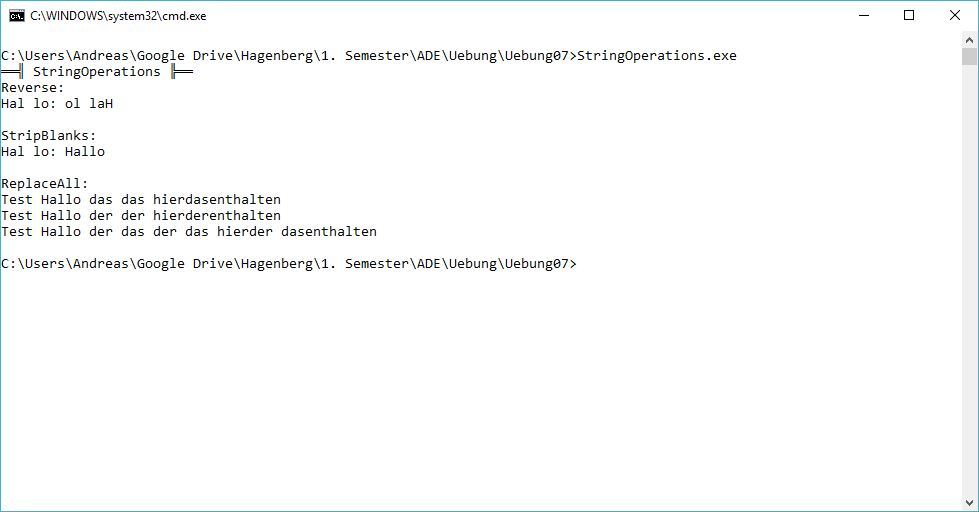
\includegraphics[scale=0.6]{./pictures/StringOperations.png}
	\caption{Testfälle Reverse, StripBlanks, ReplaceAll}
	\label{fig: String Operationen}
\end{figure}

\section*{Testfälle}
Bei Reverse wird der umgekehrte String ausgegeben.
StripBlanks zeigt das Leerzeichen aus einem String entfernt werden.
Bei ReplaceAll wird zuerst ein String durch einen komplett anderen ersetzt.
Die zweite Ausgabe zeigt das das ersetzen auch funktioniert wenn der neue String gleich ist mit dem alten oder der alte String in dem neuen enthalten ist.

\newpage

\subsection*{Aufgabe 2}
\subsubsection*{Lösungsidee}
Die Plausibilitätsüberprüfung von Messwerten kann auf verschiedene Arten gelöst werden.
Die drei hier verwendeten Arten:
\begin{itemize}
\item Globale Variablen
\item Lokale Variablen
\item Unit
\end{itemize}
Bei Globalen Variablen ist der große Nachteil/Vorteil das sie überall im Programm verwendet werden können. Bei Lokalen Variablen ist der Nachteil das sie nur innerhalb des Hauptprogrammes verwendet werden können. Die Unit verwendet ihre eigenen Variablen und greift auch selbst auf diese zu. Damit kann ohne Variablen Initialisierung im Hauptprogramm trotzdem ein Messwert überprüft werden. Alle drei Arten "merken" sich die vorherige Zeit und Temperatur und überprüfen damit ob die Temperatur plausibel ist. Zusätzlich müssen bei allen drei Arten die Werte mindestens einmal initialisiert werden sonst funktioniert die Überprüfung nicht.
\newline

\lstinputlisting[language=Pascal] {../isPlausible_PseudoCode.pas}
\lstinputlisting[language=Pascal] {../temp.pas}
\begin{figure}[H]
	\centering
	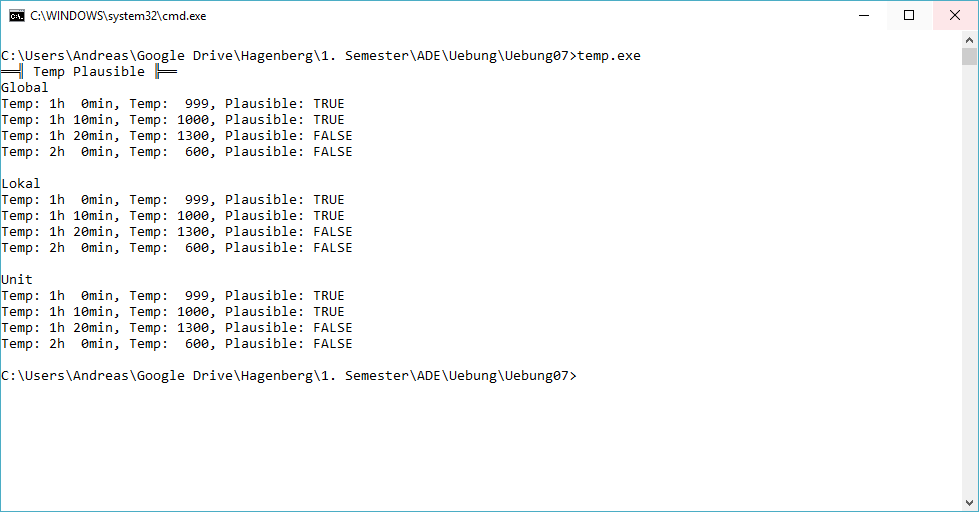
\includegraphics[scale=0.6]{./pictures/temp.png}
	\caption{Testfälle Temperatur Messung}
	\label{fig: Temp Messung}
\end{figure}

\section*{Testfälle}
Die Testfälle zeigen die Messwertüberprüfung bei allen drei Arten.
\newpage

\subsection*{Aufgabe 3}
\subsubsection*{Lösungsidee Übung 2}
Bei der Quadratwurzelberechnung soll mithilfe einer Reellen Zahl und einer Fehlerschranke die Quadratische Wurzel der Reellen Zahl berechnet werden. Dazu muss die Richtigkeit der Eingabe überprüft werden und entsprechende Fehlermeldungen ausgegeben werden. Nach der Überprüfung der Eingabe soll mithilfe der Newtonsche Iterationsformel eine Näherung für $y \approx \sqrt{x}$ berechnet werden. Mithilfe der Formel $ y1 = \frac{1}{2}(y0 + \frac{x}{y_{0}})$ und einer Repeat Until Schleife die nach 50 Iterationen abbricht wird eine Näherung für die Eingabe berechnet.
\newline
\lstinputlisting[language=Pascal] {../quadratwurzel_old.pas}

\newpage
\subsubsection*{Anmerkungen}
Für die Lösungsidee ist nicht notwendig wie diese Formel aussieht solange sie im Programm verwendet wird. Der Programmstil selbst zeichnet sich durch einen nicht eingehaltenen Standard aus, wie etwa das klein schreiben der Schlüsselwörter. Die Näherung selbst kann in eine eigene Funktion ausgelagert werden, damit kann die Funktion überall einfach verwendet werden, falls Änderungen an der Näherung gemacht werden muss somit nicht überall der Programm Code verändert werden. Die Repeat Until Schleife kann durch eine While Schleife ersetzt werden.
\newline

\subsubsection*{Lösungsidee Neu}
Mithilfe einer Prozedur und Call By Reference wird mit einer Näherungsformel die Quadratwurzel einer Zahl ausgerechnet. Wenn nach 50 Iterationen keine Konvergenz gefunden wurde wird abgebrochen. Zusätzlich werden die Eingaben auf Fehler überprüft und entsprechende Fehlermeldungen ausgegeben.
\newline
\lstinputlisting[language=Pascal] {../quadratwurzel_new.pas}
\begin{figure}[H]
	\centering
	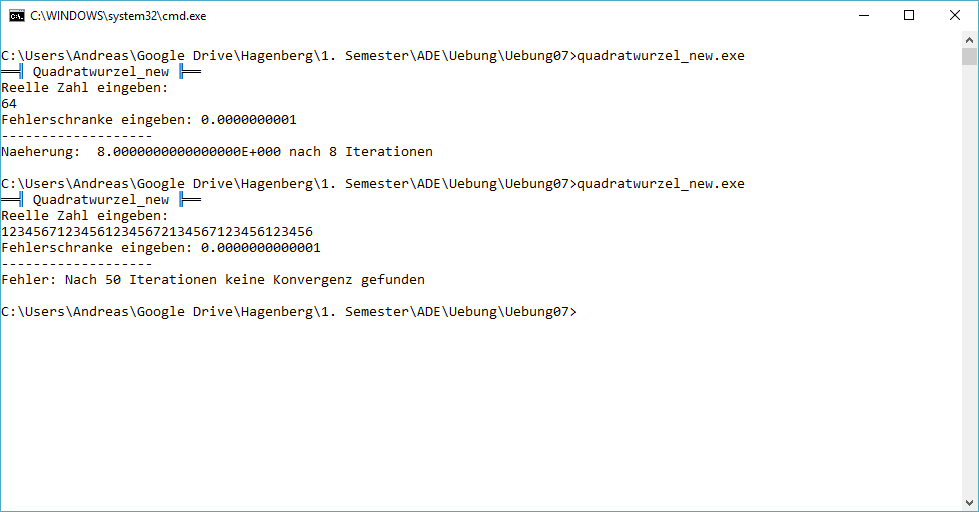
\includegraphics[scale=0.6]{./pictures/quadratwurzel_new.png}
	\caption{Testfälle Quadratwurzel}
	\label{fig: Quadratwurzel Neu}
\end{figure}

\section*{Testfälle}
Die Testfälle zeigen die Ausgabe mit der überarbeiteten Version von Quadratwurzel.

\newpage



\end{document}





